\setchapterimage[3.5cm]{mma/crab-page}
\setchapterpreamble[u]{\margintoc}
\chapter{Multi-Messenger Astronomy}
\labch{theory}
\begin{fquote}[William Shakespeare][Hamlet][1556] Though this be madness, yet there is method in it.
\end{fquote}

\emph{Multi-wavelength astronomy} seeks to understand the universe through correlations between photons of different energies. \emph{Multi-messenger astronomy} expands this concept to incorporate information from non-photon messengers, namely \emph{cosmic rays}, \emph{gravitational waves} and \emph{neutrinos}. Each messenger provides a unique view of astrophysical processes in objects.

\section{Cosmic Rays}

\emph{Cosmic Rays} were first discovered by Victor Hess in 1912, when the measured rate of ionising radiation was found to increase as a function of altitude, indicating the existece of an extraterrestrial flux `ioninsing rays' with a cosmic origin \sidecite{Hess:1912srp}. The name turned out to be a misnomer, beause cosmic rays are now known to actually consist of charged particle rather than rays. This has ultimately made studyinf cosmic rays more challenging, because such charged particles are deflected by the many magnetic fields in the universe. Thus, while we can now detect cosmic rays with relatively high precision, their arrival direction does not reveal much about their origin.

An industry of experiments have developed since the Hess balloon expeditions to measure the composition and spectrum of Cosmic Rays, as illustrated in Figure \ref{fig:CR_spectrum}. The data is well-described by an unbroken power-law up to $\sim$1 PeV, beyond which there is a spectral softening known as \emph{the knee}. This softer spectrum continues before undergoing a hardening, known as the \emph{ankle}. There is then evidence of a high-energy cutoff, sometimes dubbed \emph{the second knee} in a case of metaphor-stretching.

\begin{figure}
	\centering 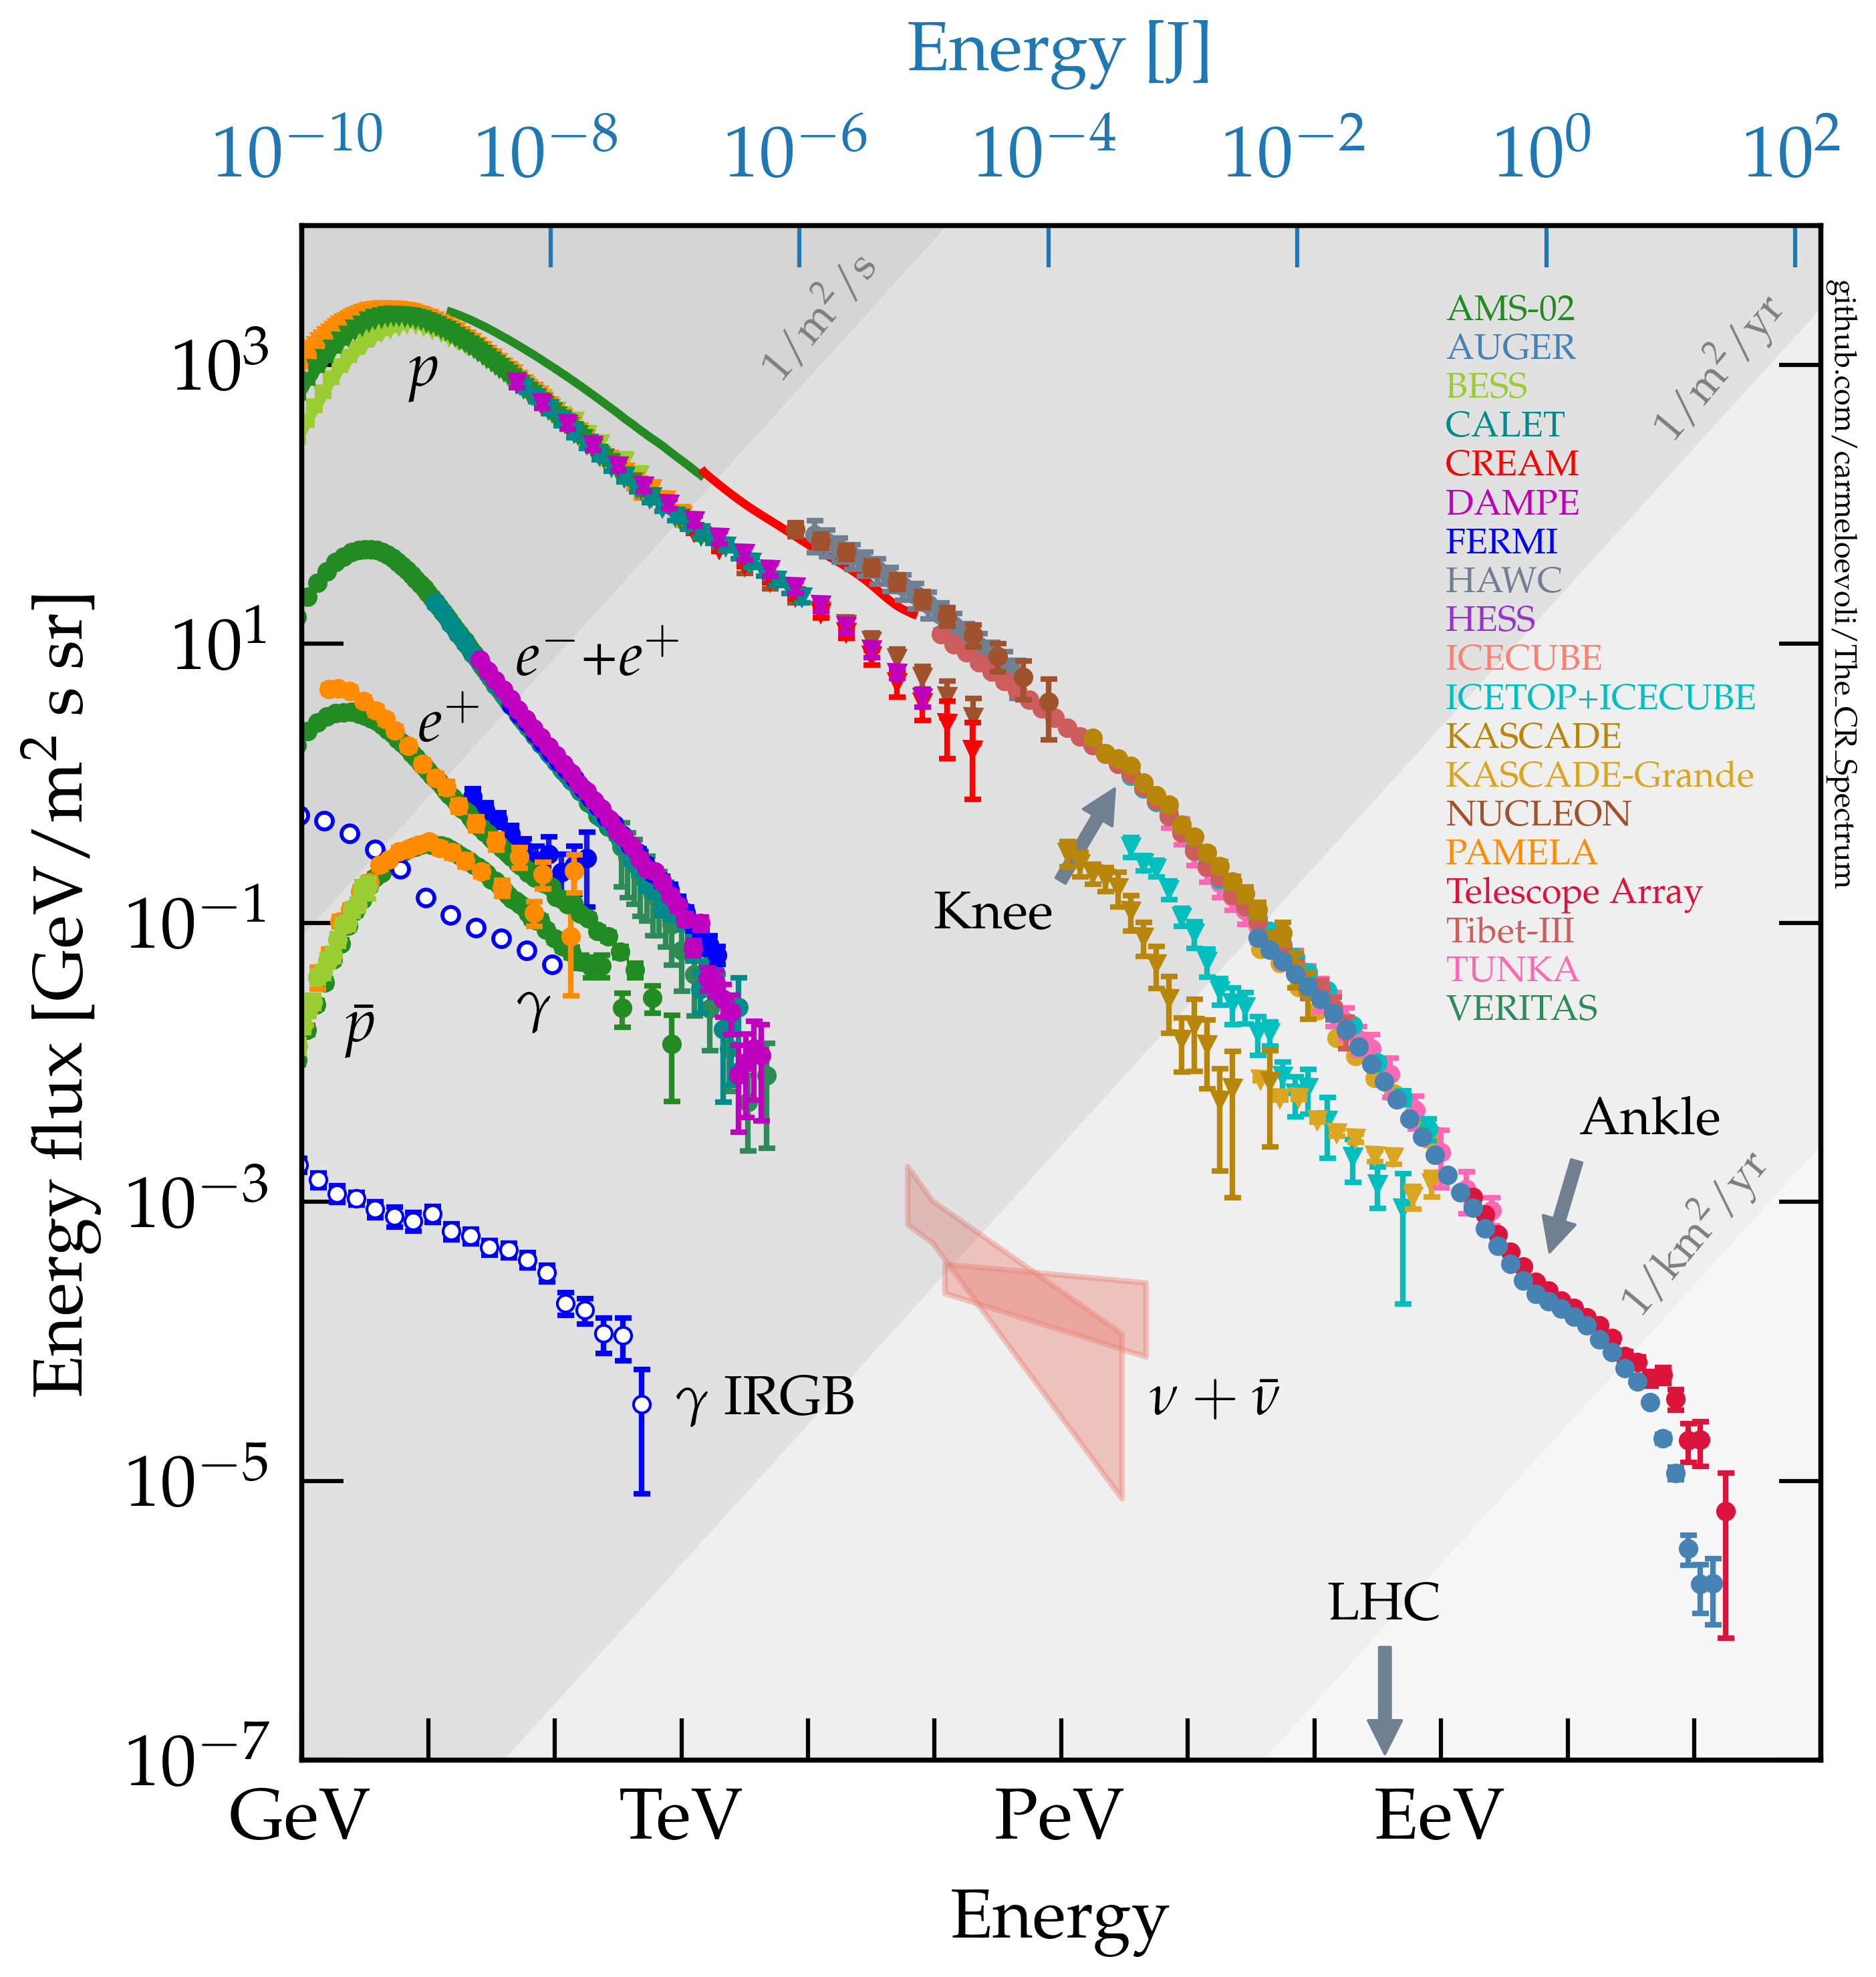
\includegraphics{mma/The_CR_Spectrum_2020}
	\caption{Cosmic Ray spectrum above 1 GeV, from \cite{evoli_carmelo_2020_4396125}.}
	\label{fig:CR_spectrum}
\end{figure}

The knee is typically identified as the point at which cosmic rays transition from being predominantly galactic to extragalactic, with the ankle component being fully extragalactic. The origin of the high-energy cutoff is unclear, and the corresponding flux is so low that detector arrays must be several hundred square kilometers to study this regime with high statistics. Events with energies >10$^{18}$ eV are named \emph{Ultra-high energy cosmic rays} (UHECRs), and today these UHECRs are primarily studied by the \emph{Pierre Auger Detector} and \emph {Telescope Array} detector. This UHECR regime is particularly interesting, because it is the point at which the so-called \emph{GZK mechanism} will begin to suppress the cosmic ray flux \sidecite{greisen_66, zk_66}. The GZK mechanism arises when comsic rays interact with ambient Cosmic Microwave Background (CMB) photons to produce a resonant $\Delta$ baryon:

In general, accelerated hadrons can interact through \emph{photohadronic} (p$\gamma$) nuclear interaction to produce pions via a resonant $\Delta$ baryon:

\begin{equation}
	p + \gamma \rightarrow \Delta^{+} \rightarrow n + \pi^{+}
	\label{eq:GZK_pip}
\end{equation}

\begin{equation}
	p + \gamma \rightarrow \Delta^{+} \rightarrow p + \pi^{0}
	\label{eq:GZK_pi0}
\end{equation}

The GZK mechanism is a specific case of pion production where $\gamma = \gamma_{CMB}$. Given that the CMB photon spectrum is fixed, Equations \ref{eq:GZK_pip} and \ref{eq:GZK_pi0} would lead to a cutoff, in which pion production suppresses ultra-high energies above a threshold energy set by the mass of the $\Delta^{+}$ resonance. Attenuation would not occur for nearby cosmic ray sources, so the presence of such a cutoff would be evidence of an \emph{an extragalatic origin} for UHECRs. 

However, the \emph{Cosmic Ray Composition} determines the exact threshold for the GZK cutoff, with heavier cosmic rays experiencing a much higher? threshold due to their higher ????. There is thus much focus on understanding whether UHECRs are proton-dominated or include a substantial iron component. A joint working group considered the recent composition measurements of PAO and TA, and concluded that they are compatible in once systematic uncertainties are accounted for \sidecite{pa_ta_17}. In general, these results support a light (proton-dominated) composition up to $\sim$10$^{19}$ GeV, above which PAO data favours a transition to a more mixed composition \sidecite{pao_composition_17}. 

An alternative explanation for any apparent cutoff is that sources of UHECRs simply cannot accelerate particles beyond certain energies due to physical constraints. In general, any cosmic ray accelerator must at a minimum satisfy the \emph{Hillas Criterion} that any particle can be contained during the acceleration process \sidecite{1984ARA&A..22..425H}. This can be calculated by equating the Lamour Radius of a particle with the physical size of an accelerator:

\begin{equation}
	\frac{E_{\textup{max}}}{\textup{PeV}} \approx
	1600 \times \frac{B}{\textup{Gauss}} \times \frac{R}{10^{16} \textup{cm}} \times
	\beta Z
	\label{eq:hillas}
\end{equation}

Equation \ref{eq:hillas} leads to a constraint on minimal magnetic field strength and source extension, which can be illustrated by a \emph{Hillas Plot} such as that in Figure \ref{fig:hillas_plot}. 

\begin{figure}[!ht]
	\centering 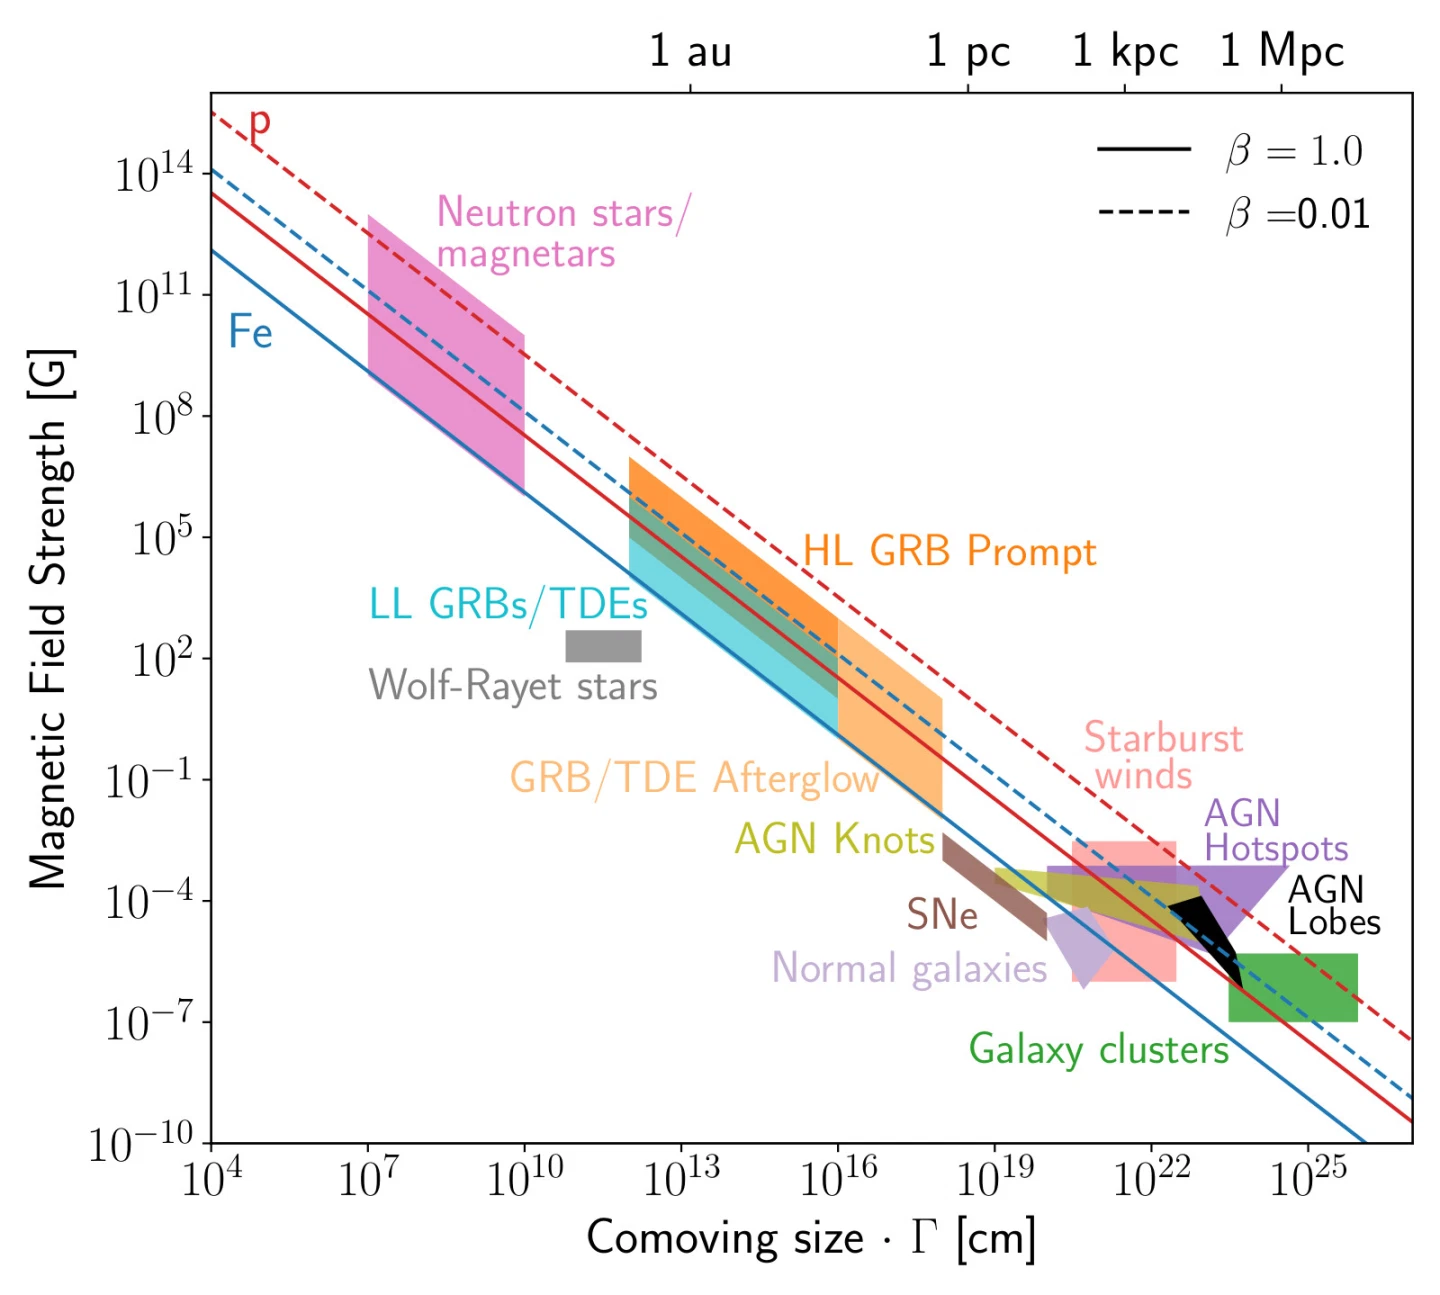
\includegraphics{mma/hillas}
	\caption{A Hillas plot illustrating possible cosmic-ray accelerators. credit: Mauricio B.}
	\label{fig:hillas_plot}
\end{figure}

The Hillas criterion is a necessary but not sufficient condition for a given source class to produce cosmic rays at the specified energy. The sources must also be capable of accelerating comsic rays to the necessary energy in the first place, and the timescale for this to occur must also be shorter than the associated particle cooling timescale. 

High-energy cosmic rays are generally though to be produced from \emph{Fermi acceleration}. Fermi acceleration is premised on the idea of `magnetic mirrors', where elastic collisions with a magnetic field leads to the deflection of a charged particle \sidecite{spurio_18}. The dominant process is thought to be \emph{First Order Fermi Acceleration}, in which acceleration occurs through repeated reflections between two magnetic fields moving closer together \sidecite{fermi_54}.

. \emph{collisionless shocks}...

In an idealised case... power law with E$^{-\gamma}$ spectrum.?$ \gamma \approx$ 2

Another contributor is \emph{Second Order Fermi Acceleration}, through which particles can be accelerated through collisions against moving magnetic fields \sidecite{fermi_49}. If the trajectory of magnetic fields were distributed randomly, collisions would preferentially occur with those trajectories moving towards the particle, and in each such collision the particle would gain energy. 

\section{Neutrinos}

The electron neutrino was first proposed as a particle by Pauli in 1930 as a solution to understand the mechanics of beta decay \sidecite{pauli_33}. Though observations suggested that the process involved a three-body decay, only the charged electron and proton could be measured. Invoking the existence of a light, chargeless particle provided a theoretical escape route:

\begin{equation}
	n \rightarrow p + e^{-} + \nu_{e}
\end{equation}

 However, this particle was proven to be more than a theoretical construct, with its existence confirmed via direct detection of \emph{beta capture} in 1956 \sidecite{cowan_56}. In parallel, the \emph{Standard Solar Model} was developed over the course of the 20th century, which correctly identified that the sun was powered by nuclear fusion \sidecite{bethe_39}. This model came with a firm prediction of a guaranteed flux of electron anti-neutrinos, \emph{solar neutrinos}, which would be produced in tandem with thermal radiation. The first attempt to measure the solar neutrino flux was by the Homestake experiment in 1964 via Cl$^{37} \rightarrow$ Ar $^{37}$, which unexpectedly detected a flux that was only one third the predicted level \sidecite{davis_68}. This deficit, dubbed the \emph{solar neutrino problem}, was subsequently confirmed by many other experiments.

The solar neutrino problem was finally resolved in 2001, when the electron neutrino deficit was conclusively matched with a corresponding excess of muon neutrinos \sidecite{sno_01}. This confirmed the presence of \emph{neutrino oscillations}, by which neutrinos can change flavour states. To undergo oscillations, neutrinos must have different non-zero mass states, in contrast to previous assumptions in the Standard Model of particle physics. 

A new generation of experiments have developed to probe neutrino flavour oscillations across a range of energies, distance baselines and detection channels. In general, \emph{reactor neutrinos} are used to probe electron neutrino disappearance, while solar neutrinos are used to probe muon neutrino appearance. Our current knowledge is summarised in N. Only the difference in squared masses can be probed by these experiments, so while it is known that mass states 1 and 2 have a difference of neV, and 13 $\sim$neV, the absolute ordering could be either \emph{Normal ordering} (m1<m2<m3) or \emph{inverted ordering} (m3<m1<m2). Directly measuring these masses remains a particle physics aim, with recent experiments such as KATRIN probing the sub-eV regime. IceCube has provided the first evidence of neutrino oscillations over astronomical baselines, with the detection of astrophysical tau neutrinos \sidecite{stachurska_thesis}.

In 1987, experiments studying the solar neutrino problem unexpectedly measured a simultaneous excess in neutrinos. This detection occurred shortly before the discovery of a nearby supernova in the \emph{Large Magellanic Clouds} (nearby dwarf galaxies orbiting the Milky Way), and coincided with the core-collapse of that supernova \sidecite{sn1987a_neutrino}. These \emph{supernova neutrinos} were the first that could be cleanly identified as arising from beyond our solar system, and confirmed the essential \emph{neutrino cooling} that occurs during the stellar core collapse (see also Chapter \ref{ch:sources}). This was also the first example of astronomy with multiple messengers. Only nearby galactic supernovae produce a sufficiently large flux to be clearly identified against detector backgrounds. However, the predicted diffuse supernova neutrino background will soon be within reach of experiments.

For this thesis, the most relevant neutrino detection method is via \emph{charged current} (CC) and \emph{neutral current} (NC) interactions of the weak force. CC interactions are mediated by W$^{\pm}$ bosons:

\begin{equation}
	\nu_{l} + N \rightarrow W^{\pm} \rightarrow l^{\pm} + X
\end{equation}

\begin{equation}
	\nu_{\mu} + N \rightarrow W^{\pm} \rightarrow \mu^{\pm} + X
\end{equation}

while NC interactions are instead mediated by Z bosons:

\begin{equation}
	\nu_{l} + \rightarrow Z \rightarrow \nu_{l} + X
\end{equation}

where l is a lepton family (e, $\mu$, $\tau$, N is a nucleon and X represents the daughter hadronic particles \cite{spurio_18}. Neutrinos are then detected indirectly via the electromagnetic signature associated with the lepton l or hadrons X, typically via the \emph{Cherenkov effect}. 

frank tamm and cherenkov here?

This detection principle is employed by km$^{3}$-scale neutrino telescopes such as IceCube (see Chapter \ref{ch:icecube} to target neutrinos at higher (GeV-PeV) energies. Interactions of cosmic rays with the atmosphere should produce a guaranteed flux of \emph{atmospheric neutrinos} at these energies, and this was confirmed observationally with the AMANDA neutrino telescope in 2002 \sidecite{amanda_02}. This flux extends over many orders of magnitude, as can be seen in Figures \ref{fig:ic_diffuse_flux} and \ref{fig:nu_spectrum}. 

\begin{figure}
	\centering 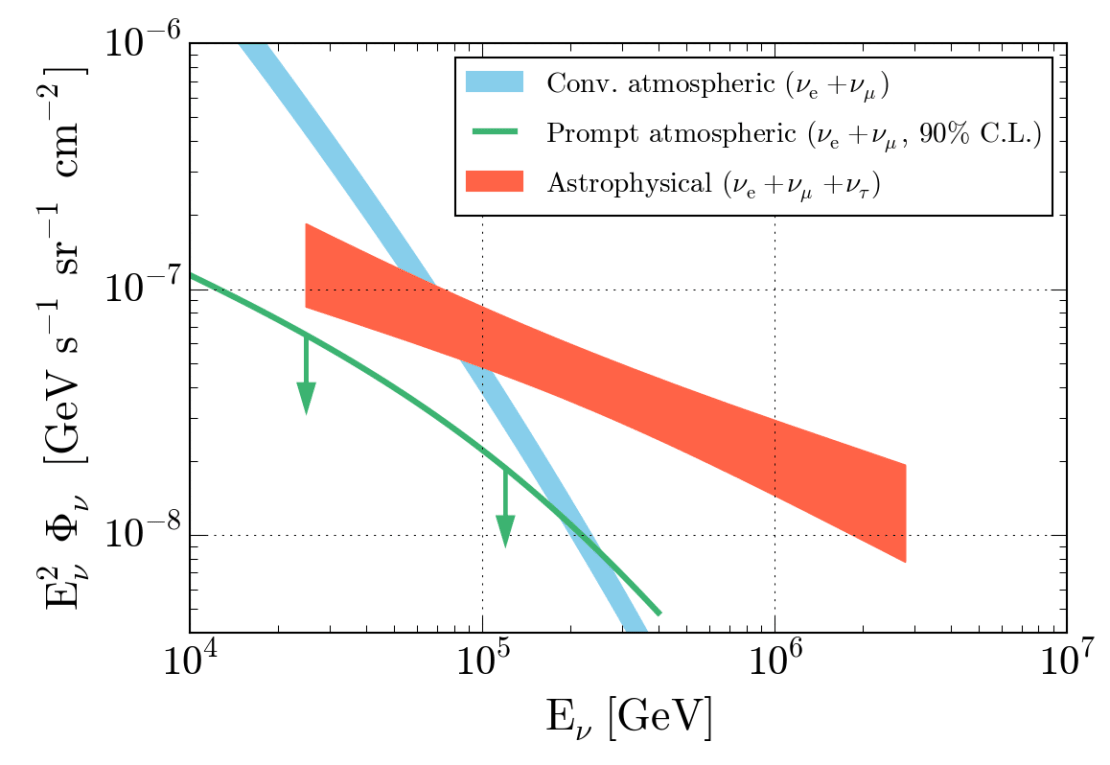
\includegraphics{icecube/ic_diffuse_flux}
	\caption{The astrophysical, atmospheric and prompt neutrino fluxes, from \cite{ic_15_joint}.}
	\label{fig:ic_diffuse_flux}
\end{figure}

\emph{Astrophysical neutrinos} (high-energy neutrinos from astrophysical sources) are to some degree guaranteed as a byproduct of high-energy cosmic ray production, resulting via pion production from the interaction of cosmic rays with ambient matter (pp) and radiation (p$\gamma$). In addition to the photohadronic interactions introduced in Equation \ref{eq:GZK_pip}, simple collisions between accelerated protons can also lead to pion production in a process analogous to fixed-target accelerator experiments:

\begin{equation}
	p + p \rightarrow \pi^{\pm}, \pi^{0}, p, n, ...
	\label{eq:pp}
\end{equation}

where higher-mass baryons and hadrons can also be produced \cite{spurio_18}. In general the daughter pions from Equation \ref{eq:pp} will follow a characteristic power law inherited from the parent proton spectrum. Regardless of the production mechanism, charged pions will ultimately decay to muons, generating muon neutrinos:

\begin{equation}
	\pi^{\pm} \rightarrow \nu_{\nu} + \mu^{\pm}
\end{equation}

These muons will further decay to electrons, generating two additional neutrinos:

\begin{equation}
	\pi^{\pm} \rightarrow \nu_{\mu} + \mu^{\pm} \rightarrow \nu_{\nu} + \nu_{\mu} + \nu_{e} + e^{\pm}
\end{equation}

However, the extent of astrophysical neutrino production depends very substantially on the conditions at cosmic ray accelerators, with high fluxes requiring abundant target material for pion production. A flux of astrophysical neutrinos was first discovered by IceCube in 2013 \sidecite{ic_astro_13}, at a level close to the maximal one allowed by cosmic ray measurements \sidecite{waxman_bahcall_98}. As can be seen from the latest flux measurement in Figure \ref{fig:ic_diffuse_flux}, this astrophysical component begins to dominate over the atmospheric neutrinos above $\sim$100 TeV. No neutrino source class has yet been detected at the 5$\sigma$ level, but possible sources of these astrophysical neutrinos are discussed further in Chapter \ref{ch:sources}.

It is expected that there should be a distinct second atmospheric component of \emph{charm} or \emph{prompt atmospheric neutrinos}, generated from the decay of charm mesons which are produced through interactions of cosmic rays with atmospheric nuclei \cite{spurio_18}. This component has not yet been measured, but as can be seen in Figure \ref{fig:ic_diffuse_flux} it remains subdominant relative to the astrophysical flux.

At the very highest energies, it is expected that the impact of the GZK cutoff (Equations \ref{eq:GZK_pip}) should generate a flux of neutrinos through interactions of UHECRs with the cosmic microwave background. These \emph{Cosmogenic Neutrinos} have not yet been observed, but upcoming radio neutrino observatories in particular are seeking to measure them. The flux of cosmogenic neutrinos depends very strongly on the composition, density and evolution of cosmic ray sources, so it remains unclear whether it will be accessible to these detectors.

\begin{figure}[!ht]
	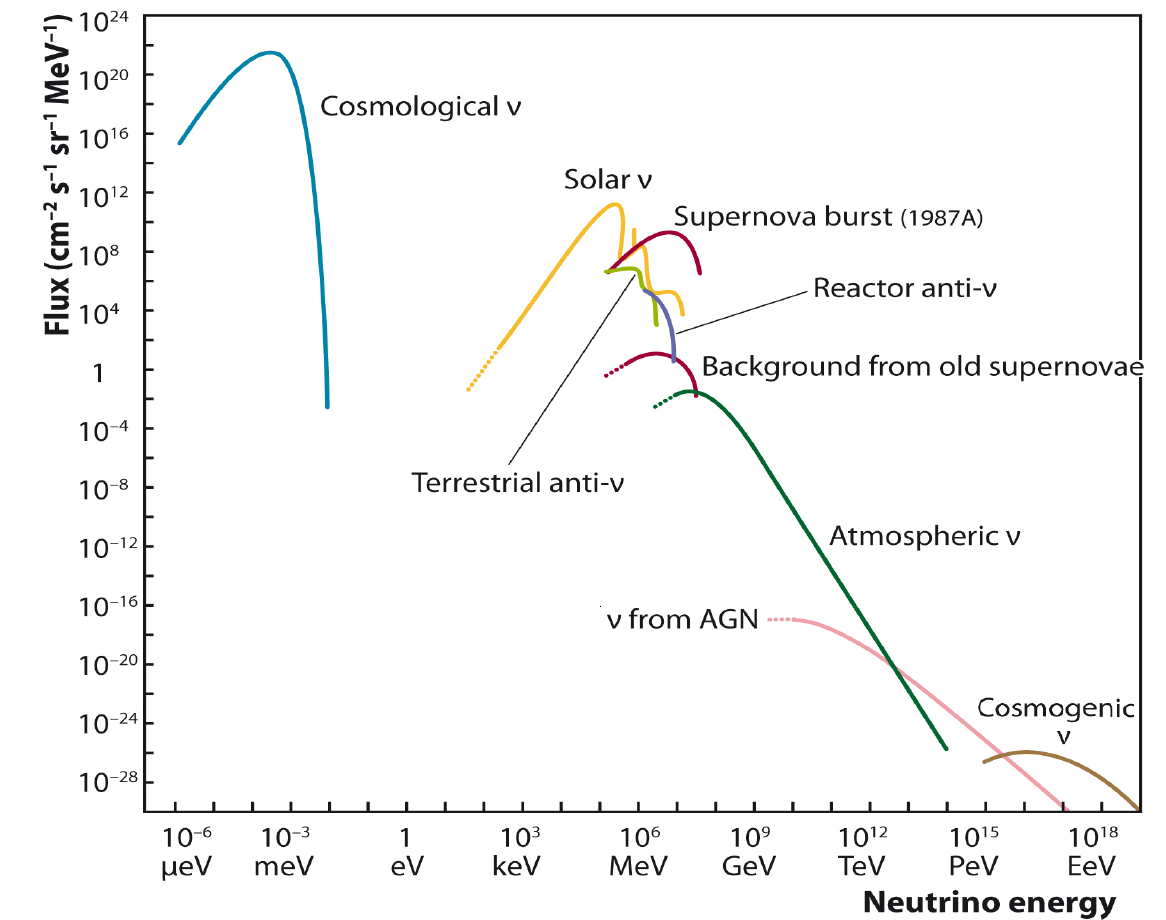
\includegraphics{mma/nu_spectrum}
	\caption{The full spectrum of neutrinos, from all sources. Credit: IceCube}
	\label{fig:nu_spectrum}
\end{figure}

\begin{figure}[!ht]
	\centering 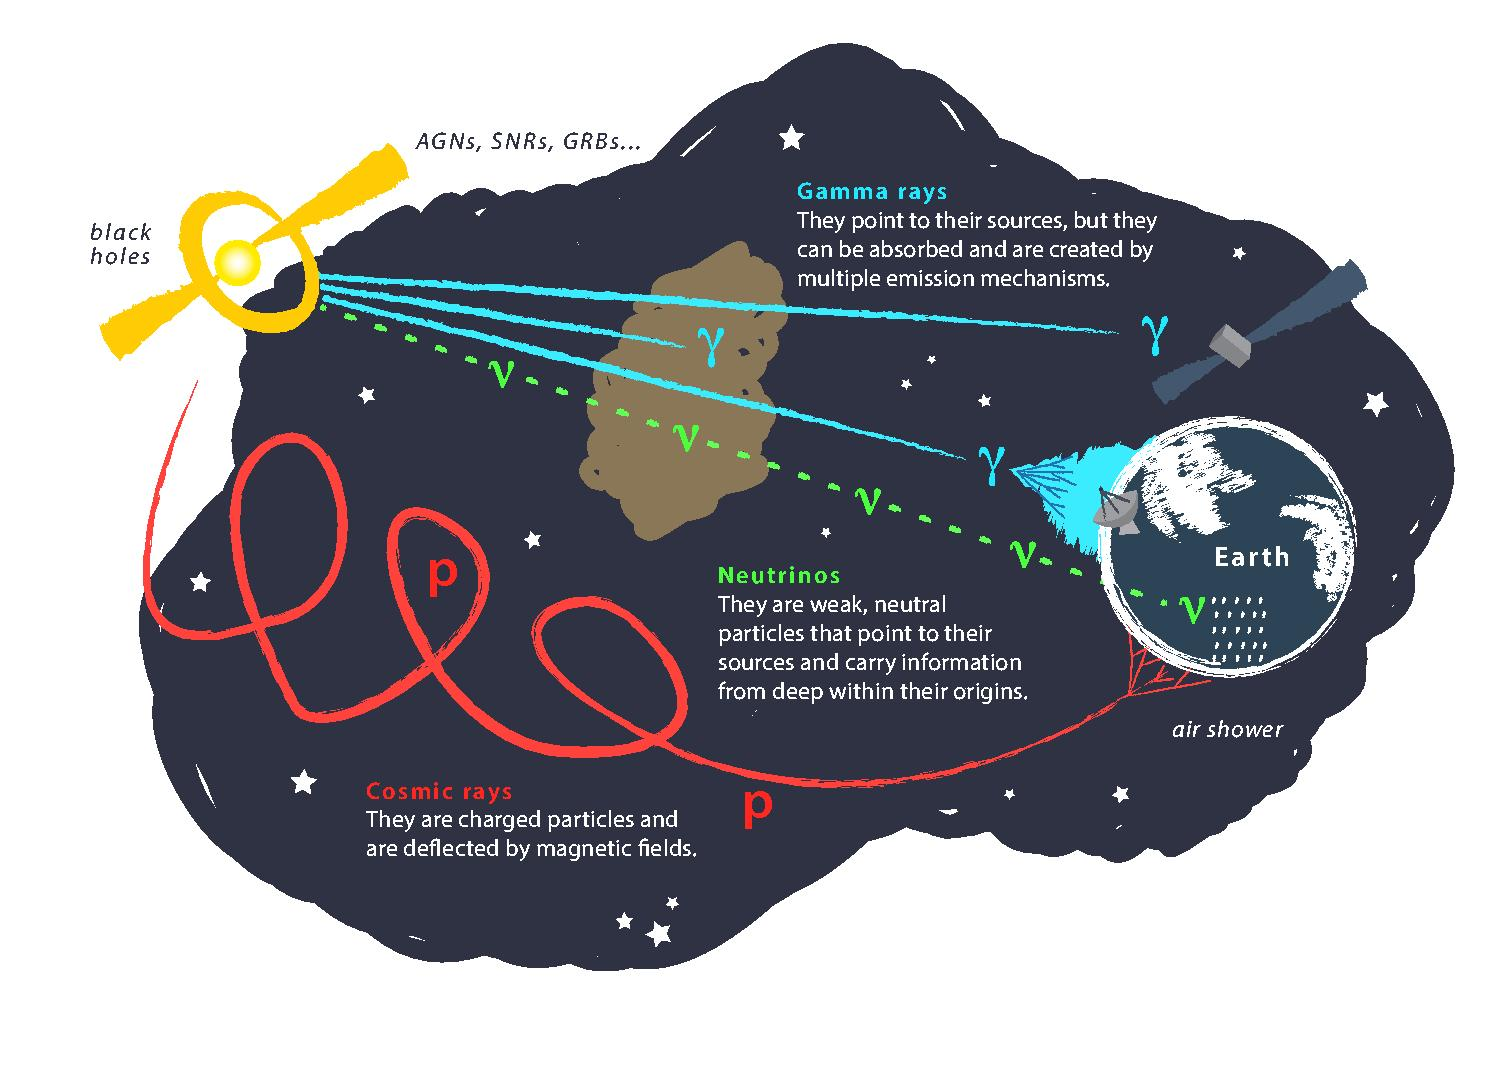
\includegraphics{mma/mm}
	\caption{An overview of multi-messenger astronomy. credit: IceCube.}
	\label{fig:mm}
\end{figure}

\section{Photons}

\begin{marginfigure}
	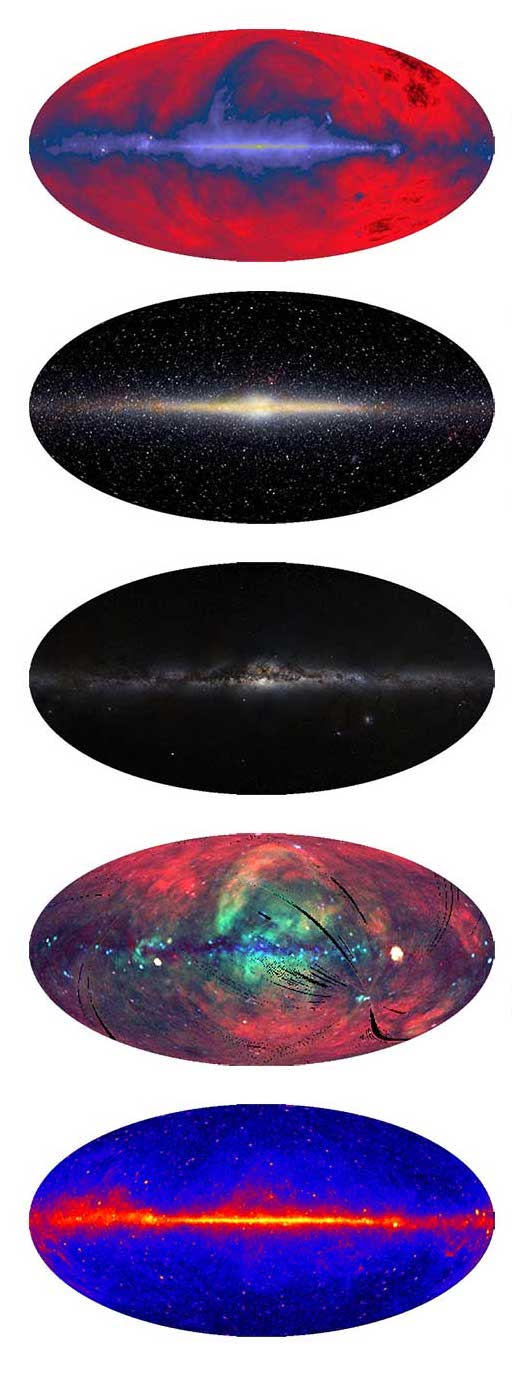
\includegraphics{mma/multiwavelength_sky_full}
	\caption{The sky, in galactic coordinates. From top: radio, infra-red, optical, X-ray and gamma-ray. Credit: NASA}
	\label{fig:mwsky}
\end{marginfigure}

Photon astronomy, in particular that in optical wavelengths, is the oldest branch of astronomy. As clear in Figure \ref{fig:mwsky}, our own galaxy is the most obvious structure at all wavelengths. The different pictures of the galaxy are also noteworthy. One example is dust extinction obscuring a large portion of the optical emission (middle panel), but  which is reprocessed to yield a particularly clear infra-red image (upper middle panel). This is an illustration of one broader principle, that interpolation between different photon energies can reveal additional information about astrophysical objects.

In general, photon emission can be divided into two broad classes, \emph{thermal emission} and \emph{non-thermal emission}. Thermal emission is approximate black-bodies, and produces characteristic spectra. Non-thermal emission arises from particle acceleration, and is typically characterised by power-law emission. Objects can have both components. Thermal emission is typically centred in IR, optical or UV wavelengths, while non-thermal emission is typically extends from low energies (radio) to high-energies (hard X-rays and gamma-rays).
 
 \subsection*{Thermal Photons}
 
 \emph{Thermal photons} are those produced by \emph{blackbody radiation}, which have a characteristic form described in \emph{Planck's Law}:
 
 \begin{equation}
 	\frac{dE}{dt d\nu dA d\Omega} \equiv B(\nu, T) = \frac{2h\nu^{3}}{c^{2}} \frac{1}{e^{h\nu/k_{b}T} -1}
 \end{equation}

where B is the \emph{Spectral radiance} of the source, $\nu$ is the frequency, and T is the temperature \sidecite{planck_01}. By integrating over the full solid angle, and accounting for redshifting (see Chapter \ref{ch:cosmology}), the observed flux on Earth can be parameterised as:

\begin{equation}
	um
\end{equation}

where R is the radius of the object, and D is the distance to it. Many of the astrophysical population introduced in Chapter \ref{ch:sources}, such as \emph{supernovae} or \emph{tidal disruption events} can be well described by such thermal spectra. With observations in multiple bands, such as optical, IR and UV, the physical properties of a source can be inferred at different observation epochs. 

Most astrophysical populations have temperatures >10$^{3}$ K and <10$^{5}$ K, meaning that a substantial fraction of the thermal emission in in the sensitive range of optical telescopes such as ZTF (see Chapter \ref{ch:ztf}). Surveys at these wavelengths are well-suited to first identify such objects for use e.g in neutrino astronomy, even though this thermal emission is unrelated to the hadronic processes which accelerate particles. Having found these objects, their neutrino emission can then be studied e.g with dedicated likelihood analysis as introduced in Chapter \ref{ch:llh}. In any case, the thermal emission of such objects provides an estimate of the source bolometric luminosity, giving a scale for energy output, and also an approximate model for the photon field in the source.

 \subsection*{Spectroscopy}

While photon observations are typically integrated over relatively-wide range of wavelengths, additional information can be gleaned from \emph{high-resolution spectroscopy}, in which emission in fine wavelength bins can be analysed. With precision measurements  ..

photoelectric effect?

\emph{Emission lines} are generated through photon emission at particular nuclear resonances, and can be used to infer the chemical composition of astrophysical objects. The exact energy is fixed by differing electron energy levels, and this produces a characteristic sequence of emission lines at different energies corresponding to different energy transitions. The most abundant sequence is the \emph{Hydrogen lines}, alternatively named the \emph{Balmer series}.

Identified emission lines can be used to infer \emph{redshift}, by comparing the observed wavelength of emission to the expected one, giving a measurement of distance to astrophysical objects. It can also be used for classification, with the temporal evolution of emission lines being the prime method to distinguish astrophysical populations. An example spectrum is shown in Figure X....

 \subsection*{Non-Thermal Photons}
 
\emph{Non-thermal photons} are those produced by accelerated particles through various cooling processes. Given its connection to accelerated charged particles, this non-thermal emission is most relevant for identifying sources of cosmic rays and neutrinos. Inherited from the parent particle population, non-thermal emission is often characterised by power-law energy spectra.

\emph{Synchrotron radiation} is generated by populations of charged particles moving through magnetic fields, which then emit typically at radio frequencies. Given that the parent electron spectrum will often follow a power law arising from Fermi acceleration up to a maximum energy, the synchrotron radiation will also follow a power law up to a corresponding \emph{peak frequency}. Synchrotron emission scales with $\sim$E$_{e}^{2}$, modifying the observed flux spectral index relative to the parent electron one. Above the peak frequency, the lack of higher-energy electrons will lead to an exponential suppression of flux, with this break typically appearing somewhere in the IR, optical, UV or X-ray bands.

At lower energies, these synchrotron photons can be reabsorbed by the electrons, a process known as \emph{Synchrotron self-absorption} (SSA). SSA leads to a suppression in the observed synchrotron flux at Earth up to a \emph{Synchotron self-absorption frequency} which depends primarily on magnetic field strength, above which the synchrotron emission is detected unattenuated. 

phase space for interaction decreases with e of the photon

Synchrotron spectra at radio wavelengths are thus well-described by broken power law models with a characteristic SSA spectral break, with the break frequency and power law indices then being used to infer the physical properties of the synchrotron-emitting region.  This procedure of particular relevance to this thesis (see Chapter \ref{ch:bran}). 

Non-thermal electrons will also generate photons at higher energies, leading to \emph{leptonic gamma-rays}. High-energy photons can be generated by \emph{Inverse Compton Scattering} (IC), in which the electrons scatter off photons and transfer energy:

\begin{equation}
	e^{-} + \gamma \rightarrow e^{-} + \gamma'
\end{equation}

where outgoing photon energy outgoing, $\gamma'$, is larger than the incoming photon energy $\gamma$. In general, extensive leptonic gamma-ray emission can be produced in astrophysical objects through \emph{Synchrotron Self-Compton} (SSC) mechanism. In this case, an accelerated population of electrons generate abundant photons through synchrotron emission, and this same electron population then upscatters these photons to higher energies via the IC effect \sidecite{spurio_18}. Alternatively leptonic gamma-rays may be produced through IC scattering with photons from an \emph{external radiation field} (i.e not from the electrons themselves), for example thermal X-rays in AGN disks (see Chapter \ref{ch:sources}).

In addition to leptonic gamma-rays, \emph{hadronic gamma rays} are produced through the decay of neutral pions. Given that these $\pi^{0}$ are always produced alongside charged pions, neutrino production must always be accompanied by a flux of hadronic gamma-rays. In principle, this can provide a photon tracer for neutrino sources. The neutral pions generated in Equations \ref{eq:GZK_pi0} and \ref{eq:pp}, will subsequently decay to a photon pair:

\begin{equation}
	\pi_{0} \rightarrow \gamma + \gamma
\end{equation}

with the photon energy lying in the gamma-ray range. However, these can be subsequently absorbed, so neutrinos may be produced in seemingly gamma-dark sources. Just as for neutrinos, pp gamma-rays will follow a characteristic power law spectrum, while for p$\gamma$ the spectrum will be more peaked.

One key challenge for gamma-ray astronomy is distinguishing between leptonic emission and hadronic emission. While lower energy (i.e radio) emission is generally leptonic, it is hard to distinguish between leptonic, hadronic or mixed lepto-hadronic emission at higher energies. Given this degeneracy, we cannot infer the existence of a flux of accompanying neutrinos merely because of a gamma-ray detection.

In any case, even if gamma-rays escape their production site, they may not reach Earth. Above $\sim$TeV energies, gamma-rays are increasingly like to interact with photons from the \emph{Extragalactic Background Light} (EBL) which pervades the universe, leading to \emph{pair production}: 

\begin{equation}
	\gamma + \gamma_{EBL} \rightarrow e^{+} + e^{-} 
	\label{eq:gamma_ebl}
\end{equation}

Similar to the GZK cutoff, Equation \ref{eq:gamma_ebl} leads to \emph{EBL absorption} which strongly attenuates the TeV gamma-ray flux from more distant objects. The vast majority of detected TeV gamma-ray emitters are thus located in the galaxy and local universe.
 
Pion bump

\section{Gravitational Waves}

Einstein
LIGO
LISA
other sources?
quadropole moment
supernovae
Einstein Telescope
O4

The first indirect evidence for Gravitational waves came after the discovery of \emph{PSR J1915+1606}, the first pulsar binary \sidecite{hulse_taylor}. This binary system had an 8 hour orbital period that could be precisely measured in 1975, and could continue to be observed over the subsequent decades. The orbital period duration was seen to shorten over time, consistent with expectations from General Relativity for energy loss in the form of gravitational waves \sidecite{taylor_gr}. 

The arm length of gravitational waves determines 

An alternative method for direct gravitational wave detection also involves pulsars, namely the \emph{pulsar timing method} \sidecite{pulsar_gw_method}. In this case the `lever arm' is the distance to known pulsars, with passing gravitational waves being detected via the consequent deviation in pulsar cycles. The \emph{Interational Pulsar Timing Array} (IPTA) is the most comprehensive present effort to detect such emission, with sensitivity at x frequencies \sidecite{ipta}.

Recent NANOgrav results derived from pulsar timing could in principle be consistent with expectations for an astrophysical GW background, but no discovery has yet been claimed \sidecite{nanograv}.